\section{Contexto Histórico}
\begin{frame}\frametitle{Thickness}
	\begin{figure}
		\centering
		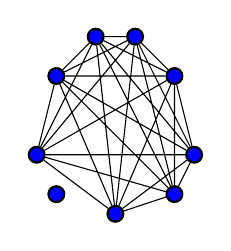
\begin{tikzpicture}
		\begin{scope}[every node/.style={circle,thick,draw,fill=blue,minimum size=2mm,inner sep=0pt}]
		\node (p1) at (0,0){};
		\node (p2) at (0.25,1) {};
		\node (p3) at (0.75,1.5){};
		\node (p4) at (1.25,1.5) {};
		\node (p5) at (1.75,1) {};
		\node (p6) at (2,0){};
		\node (p7) at (1.75,-0.5) {};
		\node (p8) at (1,-0.75) {};
		\node (p9) at (0.25,-0.5) {};
		\end{scope}
		\draw \foreach \k [count=\j from 1] in {1,...,8}
		\foreach \kk in {\j,...,8}
		{(p\k)--(p\kk)};
		\end{tikzpicture}
		\quad\quad\quad
		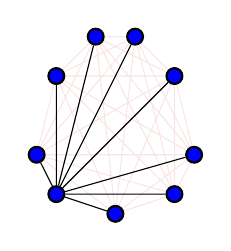
\begin{tikzpicture}
		\begin{scope}[every node/.style={circle,thick,draw,fill=blue,minimum size=2mm,inner sep=0pt}]
		\node (p1) at (0,0){};
		\node (p2) at (0.25,1) {};
		\node (p3) at (0.75,1.5){};
		\node (p4) at (1.25,1.5) {};
		\node (p5) at (1.75,1) {};
		\node (p6) at (2,0){};
		\node (p7) at (1.75,-0.5) {};
		\node (p8) at (1,-0.75) {};
		\node (p9) at (0.25,-0.5) {};
		\end{scope}
		\draw[red!80!black,opacity=0.1] \foreach \k [count=\j from 1] in {1,...,8}
		\foreach \kk in {\j,...,8}
		{(p\k)--(p\kk)};
		\draw \foreach \kk in {1,...,8}
		{(p9)--(p\kk)};
		\end{tikzpicture}
	\end{figure}
	En 1961, Harary propone un problema:
	\begin{quotation}
		Demuestre la siguiente conjetura: Para cualquier gráfica $G$ con 9 vértices, $G$ o su gráfica complementaria $\overline{G}$\let\thefootnote\relax\footnote{$\overline{G}$:La gráfica inducida resultante de remover todas las aristas de $G$ de $K_n$} es no planar.
	\end{quotation}
	Harary, Battle y Kodoma y Tutte probaron, de manera independiente, que $K_9$ no es la unión de dos \emph{gráficas planares} (no es biplanar). En 1963, Tutte definió el \emph{thickness} de una gráfica, generalizando el término de biplanaridad. 
	\let\thefootnote\svthefootnote
\end{frame}
\begin{frame}
\frametitle{Gráfica geométrica}
Una \emph{gráfica geométrica} $\mathsf{G}=(V,E)$ es un par de conjuntos $V$ de puntos en el plano y $E$ de 
segmentos de recta que unen pares de puntos de $V$. Llamamos vértices y aristas a estos conjuntos,
respectivamente. Una gráfica geométrica es \emph{completa} si contiene a todas las 
aristas entre pares de vértices de $V$.
\begin{figure}
	\centering
	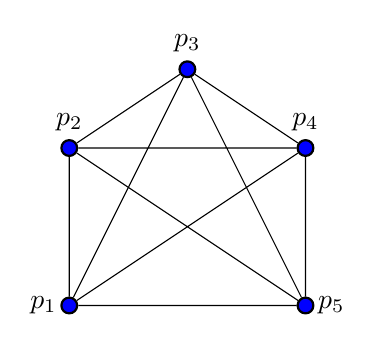
\begin{tikzpicture}
	\begin{scope}[every node/.style={circle,thick,draw,fill=blue,minimum size=2mm,inner sep=0pt}]
	\node[label=left:{$p_1$}] (p1) at (0,0){};
	\node[label={$p_2$}] (p2) at (0,2){};
	\node[label={$p_3$}] (p3) at (1.5,3){};
	\node[label={$p_4$}] (p4) at (3,2) {};
	\node[label=right:{$p_5$}] (p5) at (3,0) {};
	\end{scope}
	\draw \foreach \k [count=\j from 1] in {1,...,5}
	\foreach \kk in {\j,...,5}
	{(p\k)--(p\kk)};
	\end{tikzpicture}
	\caption{En esta gráfica geométrica $V=\{p_1,p_2,p_3,p_4,p_5\}$ y $E=\{(p_1,p_2),(p_1,p_3),\dots,(p_4,p_5)\}			$. Esta gráfica geométrica es completa.}
\end{figure}
\end{frame}
\begin{frame}\frametitle{Thickness Geométrico}
	\begin{itemize}
		\item[] Entonces podemos definir el thickness $\theta(G)$ de una gráfica $G$ como el mínimo número de gráficas planares en una descomposición de $G$. 
		
		\item[] Y el thickness geométrico $\bar{\theta}(G)$ como el número mínimo de gráficas \emph{planas} que existen en una descomposición de $G$, para todos los \emph{dibujos geométricos} de $G$.
		
		\item[] En el año 2000, Dillencourt \emph{et al.} dan el valor exacto del \emph{thickness geométrico} para gráficas completas.\\[5pt]
	\end{itemize}
	
\end{frame}
\begin{frame}
	\begin{figure}
		\centering
		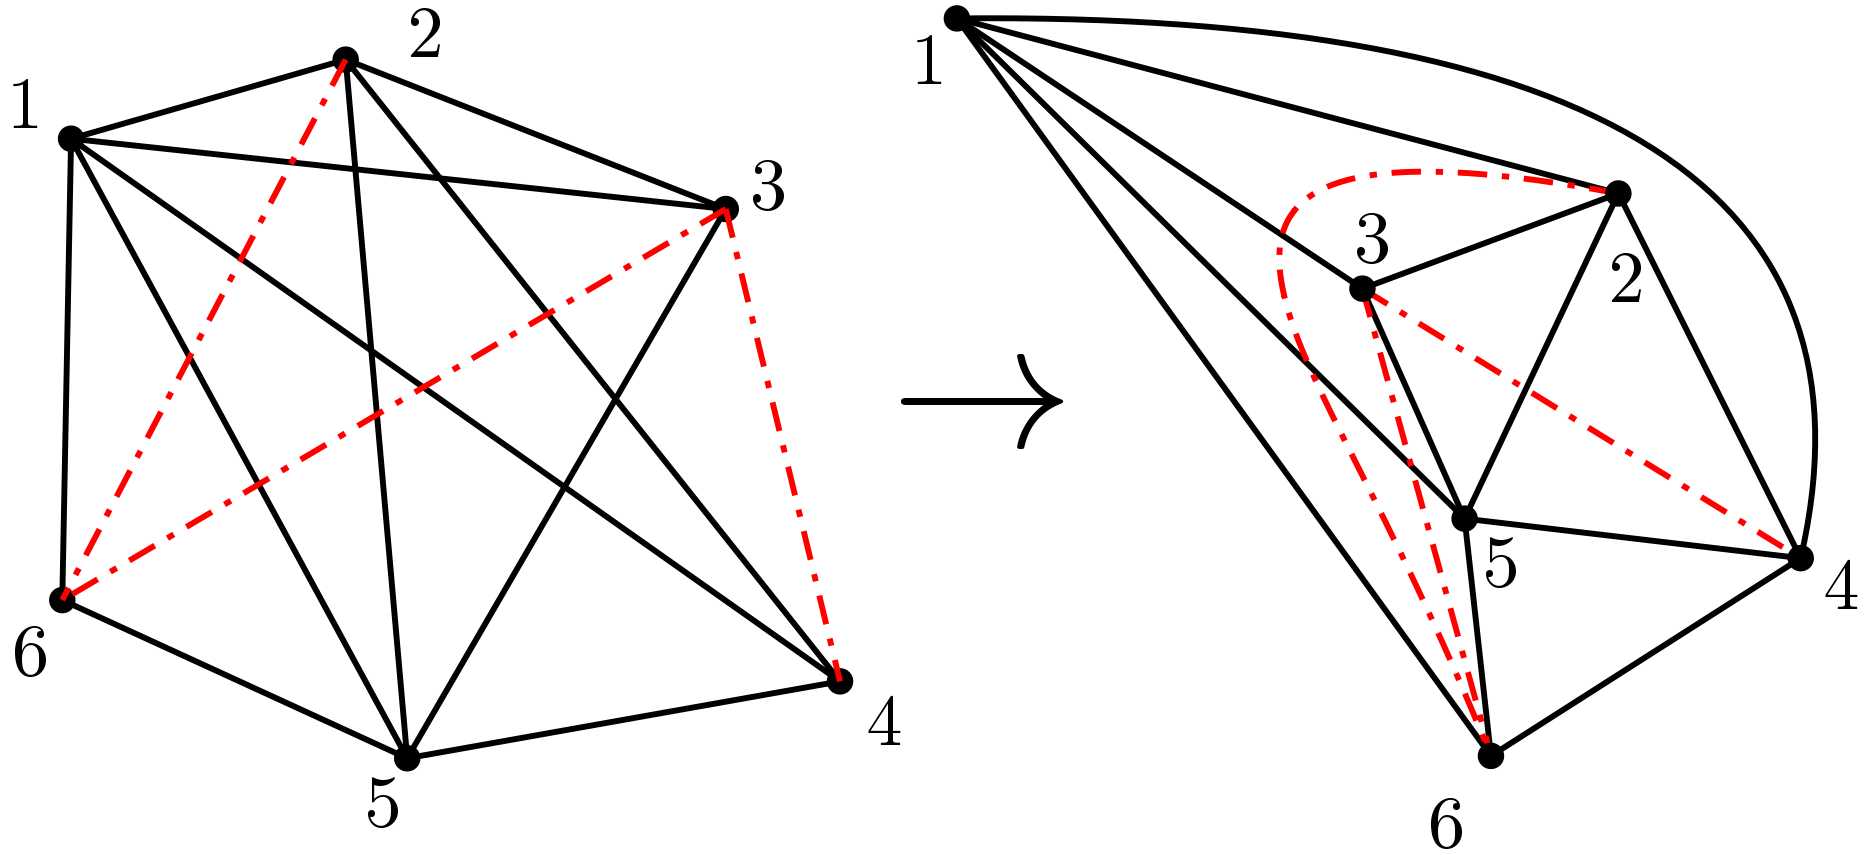
\includegraphics[width=0.6\textwidth]{images/K6_thicknes2}%
		~\vrule
		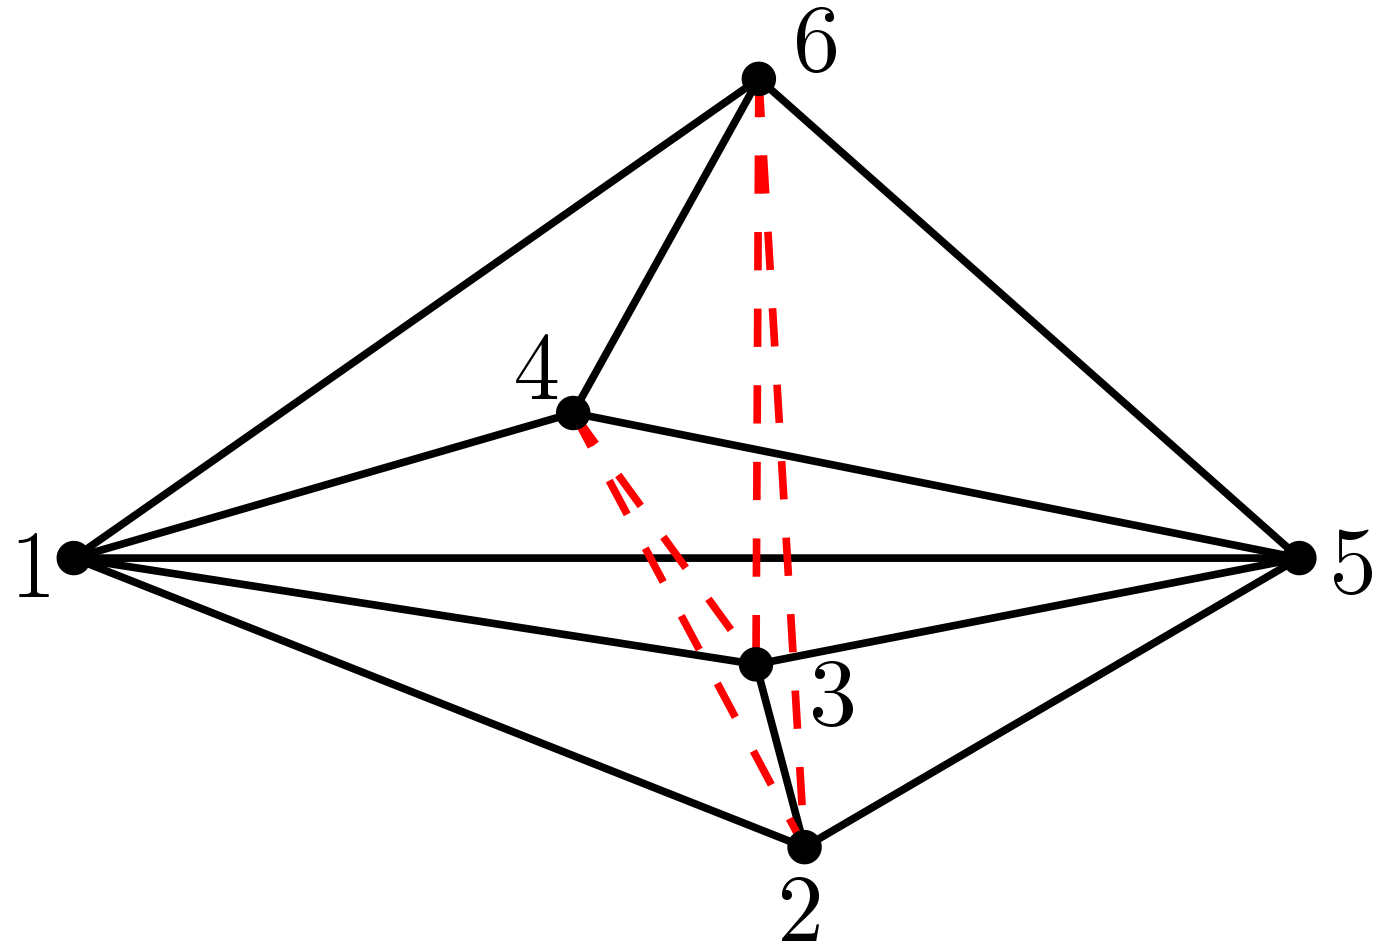
\includegraphics[width=0.4\textwidth]{images/K6_gthicknes2}
	\end{figure}
\end{frame}

\begin{frame}\frametitle{Gráfica de cruce}
Nosotros llamamos gráfica de cruce $E_{pp}(S)$ la gráfica cuyo conjunto de aristas es cada una de las aristas de $K_n(S)$ y cuyo conjunto de aristas contiene la información de los cruces de $K_n(S)$. Es decir, existe una arista entre dos vértices cuando sus aristas correspondientes en $K_n(S)$ se cruzan.
\end{frame}

\begin{frame}
\begin{figure}
	\centering
	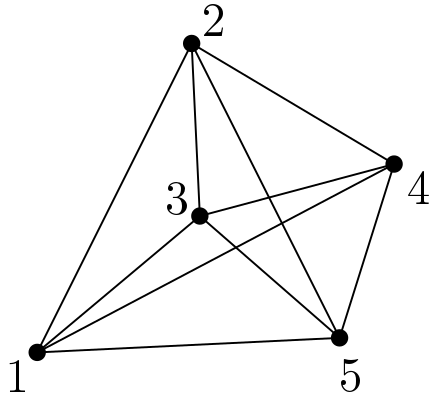
\includegraphics[width=0.2\textwidth]{images/K5}%
	~\vrule
	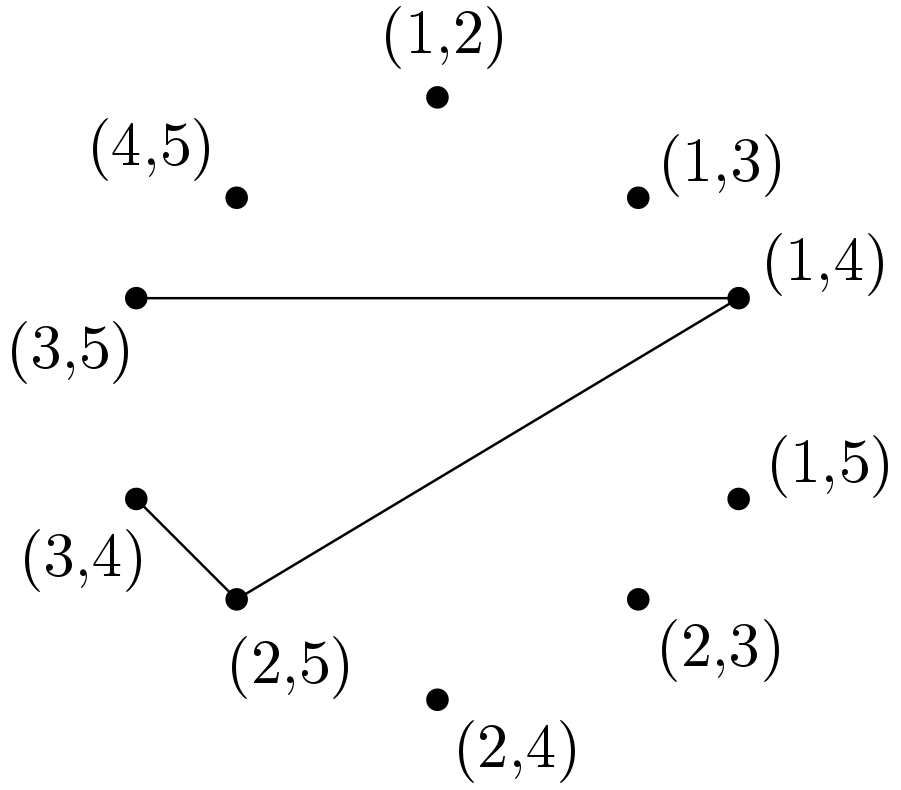
\includegraphics[width=0.3\textwidth]{images/EppK5}
	~\vrule
	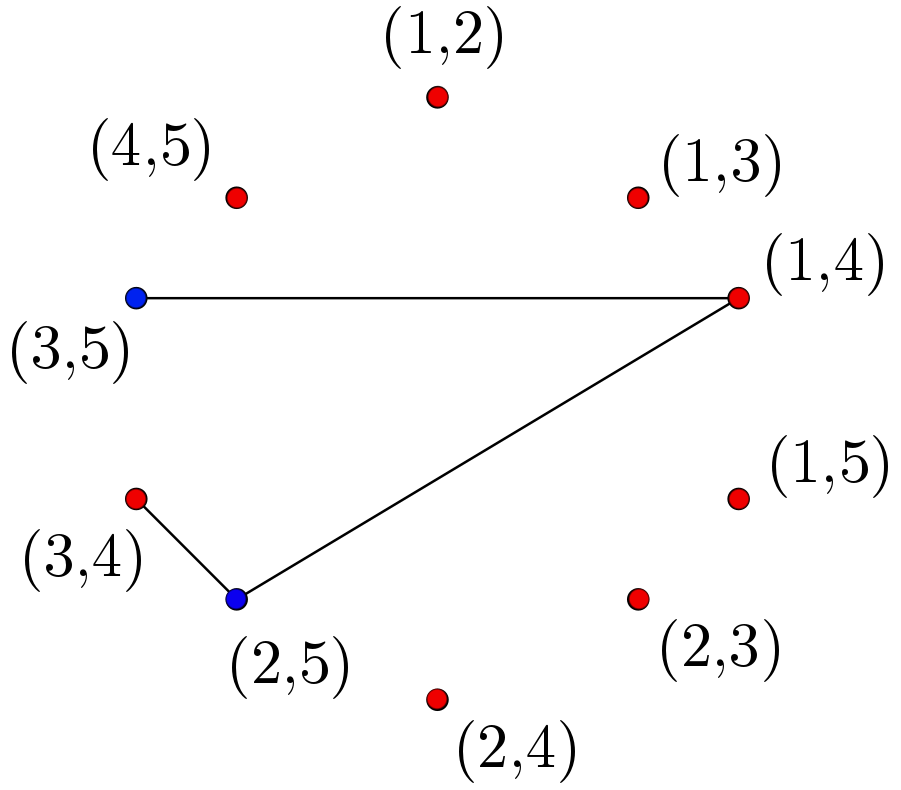
\includegraphics[width=0.3\textwidth]{images/EppK5_colored}
\end{figure}
Si encontramos una coloración propia de $C(S)$ las clases cromáticas representan gráficas planas. Luego, el número cromático $\chi(C(S))$\let\thefootnote\relax\footnote{El número cromático, $\chi(G)$, de $G$ es el mínimo número de clases cromáticas en una coloración propia de $G$.} nos dice el mínimo número de gráficas planas que hay en una descomposición de $K_n(S)$.

Por lo tanto: $\overline{\theta}(K_n(S)) = \min\{\chi(E_{pp}(S)) : S \subset \mathbb{R}^2, |S| = n\}$
\end{frame}

\begin{frame}\frametitle{Gráficas de adyacencia}
Es posible codificar la información de los cruces de las aristas de una gráfica geométrica usando un tipo de gráficas a las que llamamos \emph{gráficas de adyacencia}.

\begin{itemize}
	\item Las gráficas de adyacencia tienen como conjunto de vértices a las aristas de la gráfica completa que es inducida por algún conjunto $S$ de $n$ puntos.
\end{itemize}

	Existen otras gráficas de adyacencia a parte de $C(S)$, si consideramos otro criterio para definir las aristas de cada una podemos obtener diferentes resultados.
\end{frame}

\begin{frame}{Gráficas de adyacencia}
\begin{figure}
	\centering
	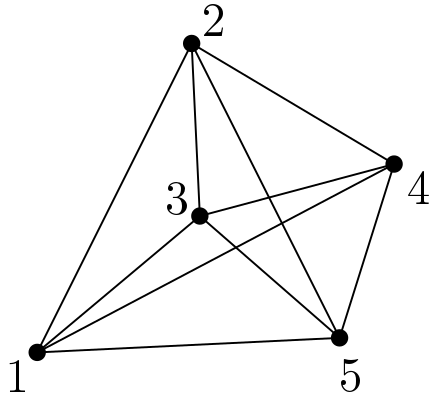
\includegraphics[width=0.2\textwidth]{images/K5}%
	~\vrule
	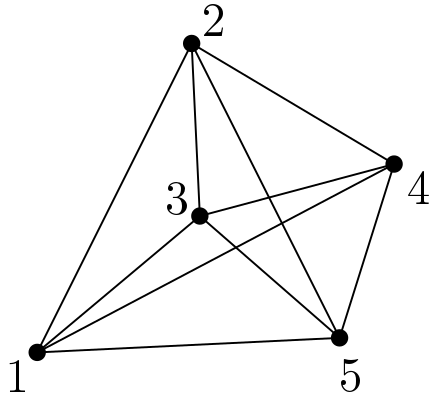
\includegraphics[width=0.2\textwidth]{images/K5}%
	~\vrule
	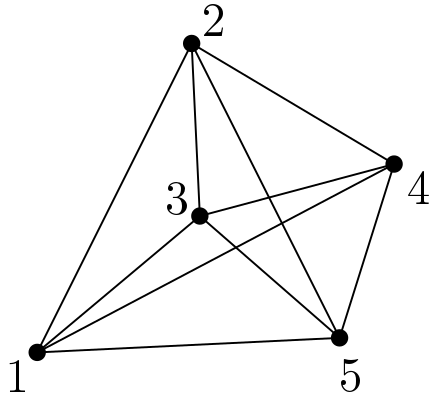
\includegraphics[width=0.2\textwidth]{images/K5}%
\end{figure}

\begin{itemize}
\item $I(S)$: Existe una arista entre dos vértices si las aristas correspondientes comparten un vértice o se cruzan. Las clases cromáticas son \emph{emparejamientos planos}.

\end{itemize}
\end{frame}
\begin{frame}{Gráficas de adyacencia}
\begin{figure}
	\centering
	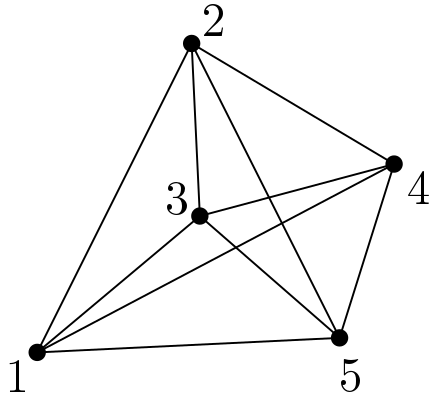
\includegraphics[width=0.2\textwidth]{images/K5}%
	~\vrule
	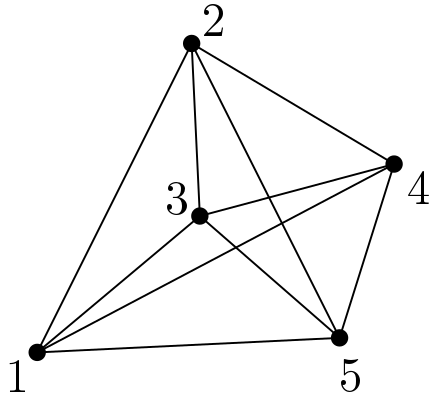
\includegraphics[width=0.2\textwidth]{images/K5}%
	~\vrule
	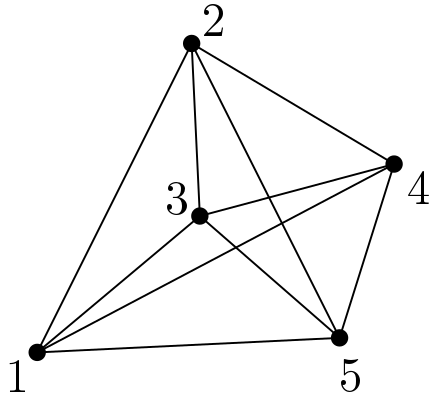
\includegraphics[width=0.2\textwidth]{images/K5}%
\end{figure}

\begin{itemize}
\item $D(S)$: Existe una arista entre dos vértices si las aristas correspondientes son disjuntas. Las clases cromáticas son \emph{thrackles}.
\end{itemize}
\end{frame}

\setbeamercovered{invisible}
\begin{frame}{Descomposiciones de gráficas}
		En 2000, Dillencourt \emph{et al.} estudiaron: 
		\[ 
			\min\{ \chi(C(S)): S \subset \mathbb{R}^2,\text{ está en posición general}, |S|=n \}
		\]
		En 2005, Urrutia \emph{et al.} estudiaron: \[\max\{\chi(G(S)): S \subset \mathbb{R}^2 \text{ está en posición general, |S|=n} \}\] donde $G(S)$ es cada una de las gráficas $W(S),I(S),D(S)$. Ellos probaron cotas para estos parámetros. En otras palabras buscan el máximo número de crossing families, emparejamientos planos y thrackles necesarios en una descomposición de $K_n$.
\end{frame}
\begin{frame}{Descomposiciones de gráficas (Book thickness)}
	Una variante del problema del thickness se basa en colocar los puntos de la gráfica completa sobre un espacio geométrico diferente del plano, específicamente sobre una recta que es compartida por un número finito de semiplanos. 
	\begin{center}
		\only<1-3>{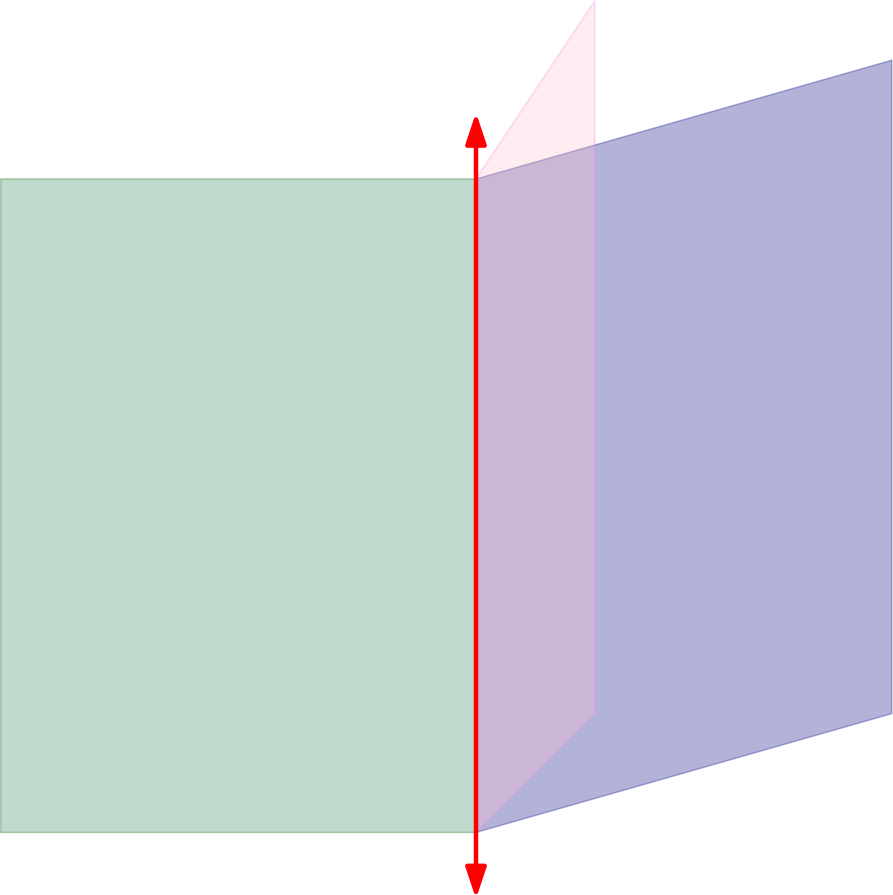
\includegraphics[width=0.4\linewidth]{images/book}}
		\only<2-3>{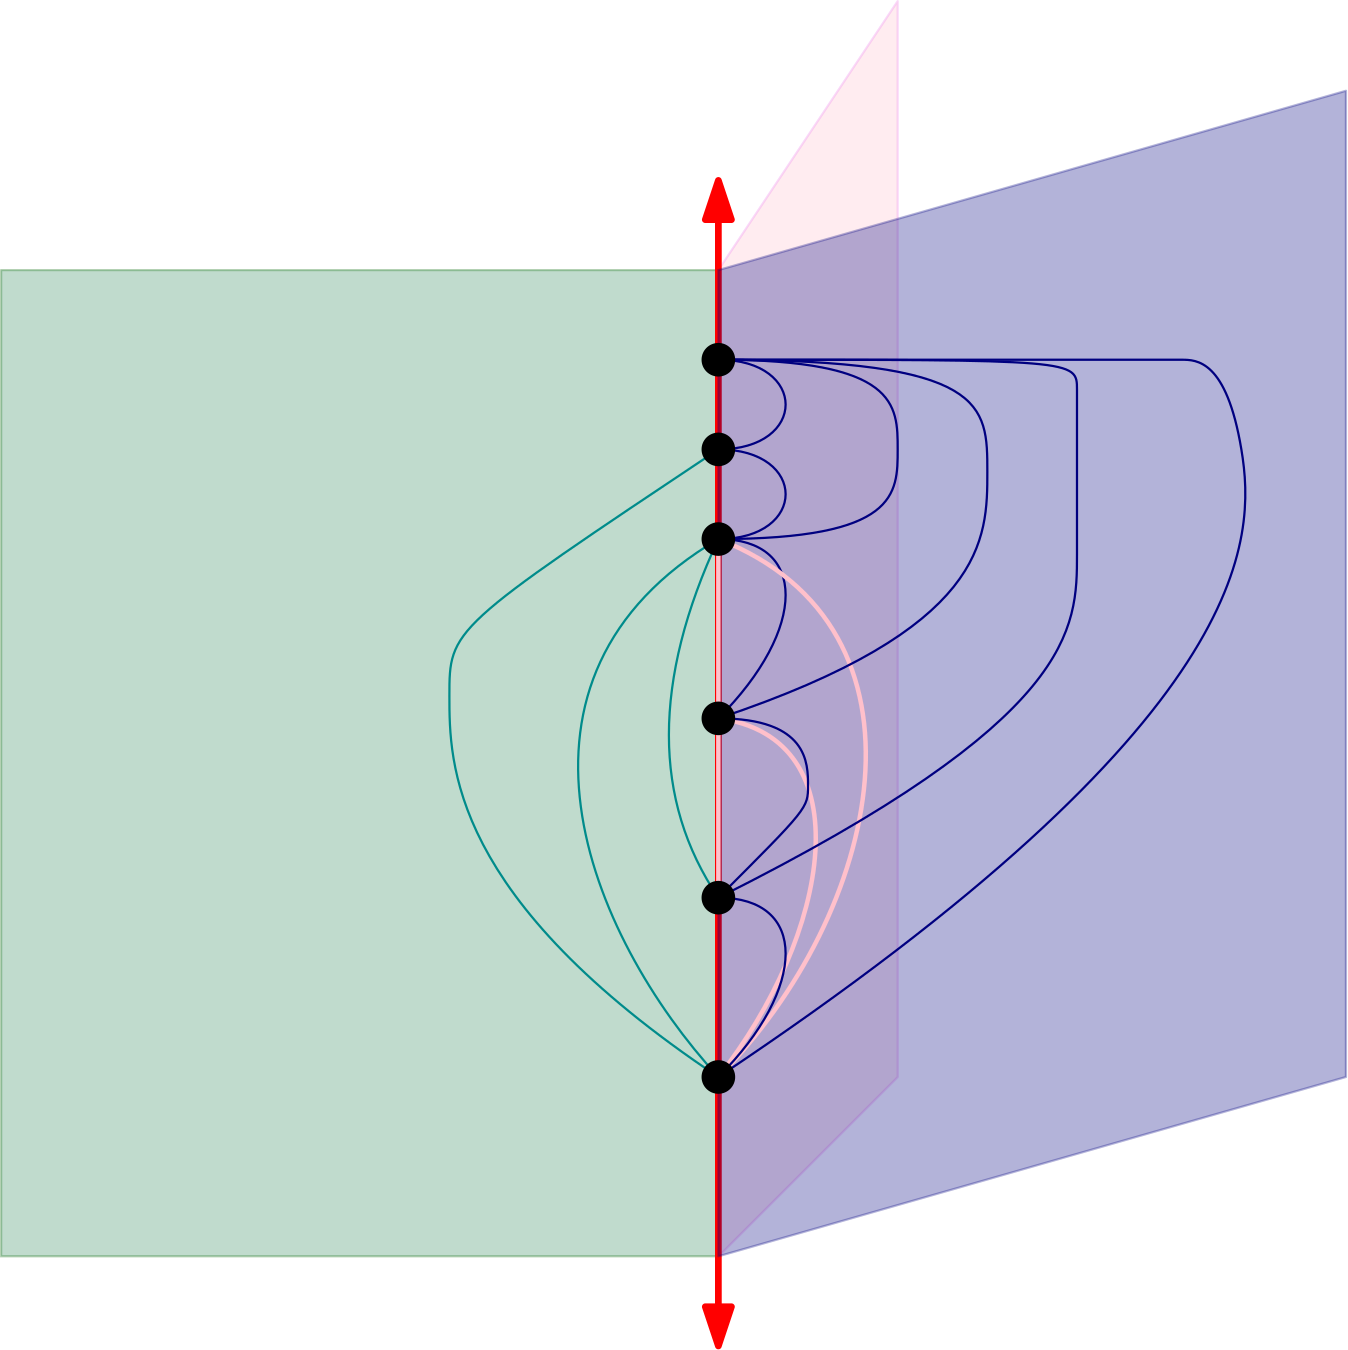
\includegraphics[width=0.4\linewidth]{images/book-thickness}}
	\end{center}
	\only<3>{
	\begin{itemize}
		\item El book-thickness es igual al thickness en posición convexa.
	\end{itemize}
	}	
\end{frame}
\begin{frame}
	\frametitle{Otras decomposiciones de gráficas}
	Solo en el plano:
	\begin{itemize}
		\item Bosques
		\begin{itemize}
			\item Star arboricity
			\item Linear arboricity
		\end{itemize}
		\item Hamiltoninan decomposition of complete graphs
		\item Cycle decomposition of complete graphs.
		\item \emph{Thrackles}
	\end{itemize}
	\begin{figure}
		\centering
		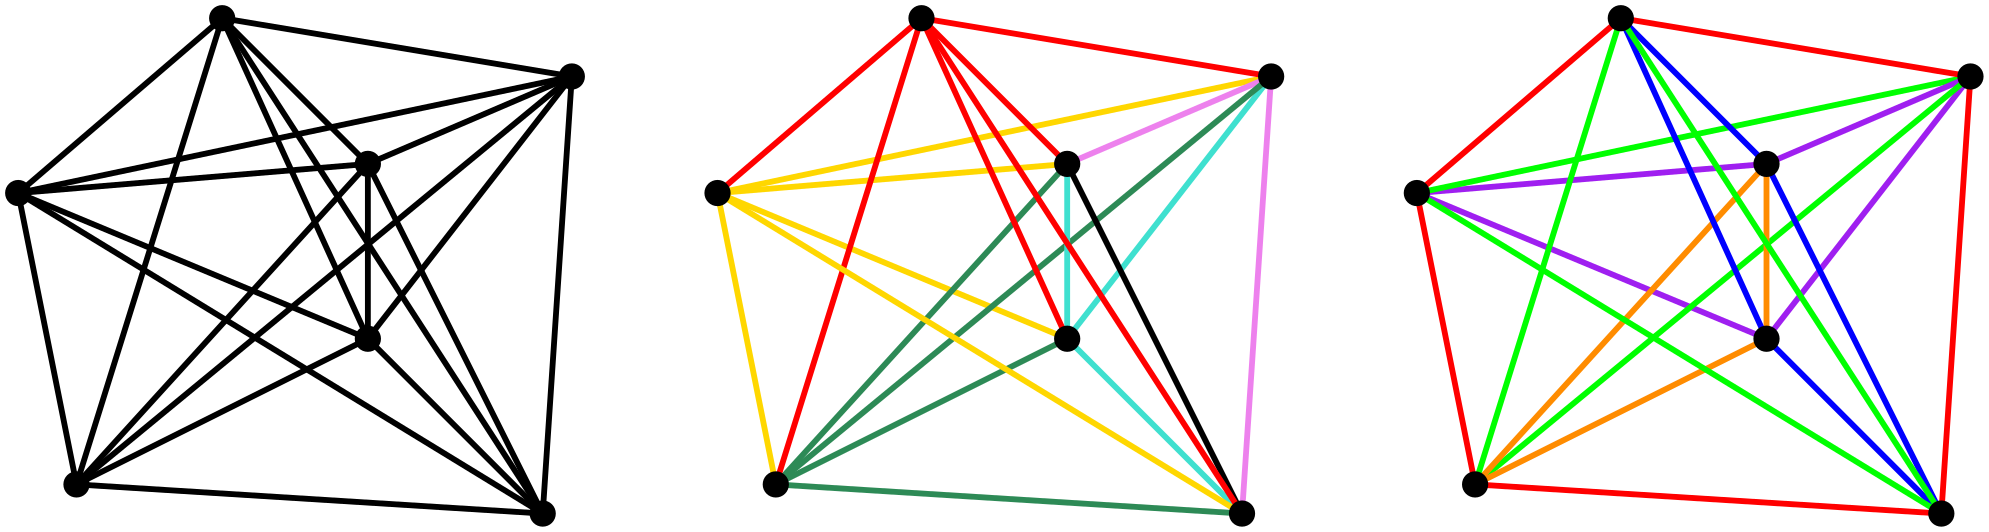
\includegraphics[width=1\linewidth]{images/other_decompositions}
	\end{figure}
\end{frame}

\begin{frame}{Anti-thickness geométrico}
\begin{itemize}
	\item Un \emph{thrackle geométrico} es un thrackle en el que cada arista es un segmento de recta.
	\item[] Sea $G$ una gráfica. El \emph{anti-thickness geométrico} mide cuántos thrackles geométricos existen, como mínimo y para todos los dibujos de $G$, en una descomposición por thrackles geométricos de $G$.
\end{itemize}

\end{frame}
\begin{frame}{Anti-thickness geométrico y el número cromático}
Recordemos que $\chi(D(S))$ nos indica cuántos thrackles geométricos hay en una descomposición de la gráfica completa inducida por $S$. 
\[
\min\{ \chi(D(S)) : S \subset \mathbb{R}^2, |S| = n \}
\] nos indica el mínimo numero de thrackles geométricos para todos los dibujos de alguna gráfica inducida por $S$, esto es, el anti-thickness geométrico.
\end{frame}




